% Editable answer content; compile CPE333_Midterm_Solutions.tex in this directory.
\sectiontitle{เฉลยและเกณฑ์ตรวจ: CPE333 Mock Midterm ชุดที่ 1}
\noindent สำหรับตรวจหลังทำข้อสอบเท่านั้น ไม่ใช่เฉลยข้อสอบจริงของรายวิชา\\คะแนนรวม 50: ปรนัย $20c/41$ เมื่อ $c$ คือจำนวนข้อถูก; เติมคำ 10; อัตนัย $8+4+8=20$\\ไม่ปัดคะแนนรายข้อ; เมื่อสรุปผลจึงปัดคะแนนรวมเป็นทศนิยมสองตำแหน่ง ไม่มีการหักคะแนนตอบผิด\par\medskip
\sectiontitle{เฉลยส่วนที่ 1: คำตอบเดียวที่ดีที่สุด}
\noindent คงถ้อยคำตัวเลือกจากข้อสอบเก่าตามต้นฉบับ; หมายเหตุด้านล่างแยกการตรวจแนวคิดออกจากการแก้ข้อความต้นฉบับ.\par
\begin{enumerate}[leftmargin=1.4em,start=1,itemsep=0.14cm]
\item \textbf{(a)} This is the option highlighted in the old exam. Technically, a trap transfers control to an OS handler; a system call may invoke a trap, so the source wording equates related but distinct concepts. {\small [L1; E09 Q1]}
\item \textbf{(c)} Without user/kernel-mode separation, a process may bypass memory protection and access another process's data. {\small [L1; E09 Q2]}
\item \textbf{(e)} The Lecture 2 model is Process = (Program, Data, Control state, Process state); all four are components. {\small [L2; E09 Q4]}
\item \textbf{(b)} Isolation protects one application from unauthorized access by another. {\small [L1; E09 Q5]}
\item \textbf{(b)} The source marks Timer interrupt and the original stem says ``non-preemptive''. Those two details conflict with the usual distinction that timer preemption is used by a preemptive scheduler; both are retained here to match the source. {\small [L2; E09 Q6]}
\item \textbf{(d)} The process descriptor/PCB is maintained in kernel space; code, data, and stack are user-space regions. {\small [L2; E09 Q7]}
\item \textbf{(c)} In the conventional layout used in the course, the stack grows opposite to the heap. {\small [L2; E09 Q8]}
\item \textbf{(d)} A process must be running before it can request I/O or another operation that blocks it; there is no direct Ready-to-Blocked transition. The source key's ``reads a file'' answer was corrected. {\small [L2; E09 Q9]}
\item \textbf{(d)} Process creation, I/O completion, and a timer-driven preemption can all place a process in the ready state in this model. {\small [L2; E09 Q10]}
\item \textbf{(d)} A zombie has terminated but remains represented until its parent collects its exit status. {\small [L2; E09 Q12]}
\item \textbf{(a)} The PCB stores per-process control information such as state and saved CPU context. {\small [L2; E09 Q13]}
\item \textbf{(a)} This is the option highlighted in the old exam. Read it as the parent still being alive after the child exits and before the parent collects the child's exit status; the printed choice is abbreviated and imprecise. {\small [L2; E09 Q31]}
\item \textbf{(e)} This is the answer indicated by the old lab question: the parent prints after the child finishes. A call to \texttt{wait()} alone does not guarantee that the child itself printed; that detail depends on the referenced lab program. {\small [L2; E09 Q14]}
\item \textbf{(d)} Two successful fork calls leave four processes to execute the print statement once each. {\small [L2; E03 Q7]}
\item \textbf{(e)} Timer preemption, blocking for I/O or wait, and yielding can each release the CPU. {\small [L2; E09 Q16]}
\item \textbf{(a)} This is the answer marked in the source. The original wording and choices are retained; interpret ``arrival order'' as selecting the next job in arrival order. {\small [L3; E09 Q15]}
\item \textbf{(b)} In the C storage-class model covered in class, \texttt{register} requests register storage for a local variable; the source's ``fastest'' claim is not guaranteed by C. {\small [L4; E09 Q19]}
\item \textbf{(c)} Fixed-size partitions can waste unused space inside an allocated partition, which is internal fragmentation. The scanned source marks this choice; a separate typed key saying ``none'' is incorrect. {\small [L4; E09 Q20]}
\item \textbf{(b)} The short-term scheduler selects a ready process to run. {\small [L3; E09 Q21]}
\item \textbf{(c)} Page replacement chooses a resident page to remove when a frame is needed. {\small [L6; E09 Q22]}
\item \textbf{(e)} Paging uses page tables, segmentation uses segment tables, and a TLB may cache translations; these mechanisms are not all required simultaneously. {\small [L5; E09 Q23]}
\item \textbf{(d)} This is the answer marked in the source. The source wording and choices are retained; note that (c), external fragmentation, is also a standard disadvantage of contiguous allocation, so the original item is not unambiguous on technical grounds. {\small [L5; E09 Q24]}
\item \textbf{(a)} Demand paging loads a page when it is referenced and is not already resident. {\small [L6; E09 Q26]}
\item \textbf{(e)} Context saving, victim selection when needed, page-in, and page-table update can all occur while handling a valid page fault. {\small [L6; E09 Q27]}
\item \textbf{(e)} The source asks which information is stored in the segment table and marks ``All choices''; Base, Bound, Direction, and Valid are the fields listed in the source. {\small [L5; E09 Q29]}
\item \textbf{(c)} With a fixed virtual address space, a larger page means fewer virtual pages and therefore a smaller page table. {\small [L5; E09 Q30]}
\item \textbf{(c)} Round robin is considered fair because it shares CPU time among active jobs on a short time scale. {\small [L3; E09 Q33]}
\item \textbf{(a)} FIFO does not use time-slice preemption; it runs the current job until completion or blocking. {\small [L3; E09 Q34]}
\item \textbf{(e)} This is the answer marked in the old exam: the memory image is kept on secondary storage. The original distractor ``virtual storage'' is retained as printed. {\small [L6; E09 Q35]}
\item \textbf{(c)} Response time is the interval from arrival until the process first gets the CPU. {\small [L3; E09 Q36]}
\item \textbf{(b)} Turnaround time is completion time minus arrival time. {\small [L3; E09 Q37]}
\item \textbf{(d)} This is the answer marked in the source. The wording is retained as printed; ``Need compacting'' refers to the compaction needed to address external fragmentation from flexible-size partitions. {\small [L4; E09 Q38]}
\item \textbf{(a)} A larger virtual address space requires more page-table entries when page and PTE sizes are fixed. {\small [L5; E09 Q39]}
\item \textbf{(e)} A multilevel page table can omit lower-level tables for unused regions; this is how it saves memory for sparse address spaces. {\small [L5; E09 Q40]}
\item \textbf{(a)} In the simplified state model used here, a newly created process is placed in the ready state. {\small [L2; E09 Q41]}
\item \textbf{(b)} A process using the processor is in the running state. {\small [L2; E09 Q42]}
\item \textbf{(e)} A long job can starve under SJF if shorter jobs keep arriving. {\small [L3; E09 Q44]}
\item \textbf{(d)} Round robin improves response time by giving each ready job a time slice promptly. {\small [L3; E09 Q46]}
\item \textbf{(d)} Pages are units of logical memory; page frames are equal-sized units of physical memory. {\small [L5; E09 Q48]}
\item \textbf{(a)} OPT is an ideal benchmark because it requires knowledge of future page references. {\small [L6; E09 Q49]}
\item \textbf{(a)} This is the option highlighted in the old exam. Read ``not valid in page table'' as a valid virtual page whose entry indicates it is not resident; strictly, an illegal virtual address is not the same as a not-present page and may cause a protection fault instead. {\small [L6; E09 Q50]}
\end{enumerate}
\newpage\sectiontitle{เฉลยส่วนที่ 2: เติมคำ / ตอบสั้น}
\noindent ข้อละ 1 คะแนน ให้ partial credit ตามองค์ประกอบในแต่ละข้อ; รับถ้อยคำอื่นที่มีความหมายถูกต้อง ไม่บังคับจำประโยคเฉลย\par\smallskip
\begin{enumerate}[leftmargin=1.4em,itemsep=.25cm]
\item \textbf{MLFQ: Multilevel Feedback Queue. STCF: Shortest Time-to-Completion First.}\\0.5 for each correct full name. Accept Multi-level and equivalent hyphenation.; สองคำย่อที่ใช้จริงใน Lecture 3 และโจทย์ scheduling ไม่ใช่คำย่ออุปกรณ์พื้นฐานเรียงหลายข้อ
\item \textbf{A program is passive code; a process is a program in execution.}\\0.5 for passive code; 0.5 for a program in execution. No resource list or additional explanation required.; Process ไม่ใช่แค่ไฟล์ program ใน disk; program เดียวมีหลาย process ได้
\item \textbf{Memory Management Unit; translates virtual addresses to physical addresses.}\\0.5 for the full name; 0.5 for virtual-to-physical translation. No protection details required.; แทนข้อ cooperative ที่ซ้ำปรนัย เพื่อเพิ่มคำย่อและความเข้าใจกลไกหน่วยความจำ
\item \textbf{Program counter (PC) and stack pointer (SP).}\\0.5 each for two distinct valid items, such as PC, SP, a general-purpose register, or the processor status register. No switching steps required.; ปรับจากแนว context switch ให้ถามเพียงตัวอย่าง 2 อย่าง ไม่บังคับอธิบายขั้นตอนเพิ่ม
\item \textbf{Process ID (PID) and process state.}\\0.5 each for two distinct non-register information types, such as PID, state, scheduling information, or memory-management information. No PCB expansion required.; ถามข้อมูล 2 ประเภท ไม่ถามชื่อเต็มพ่วงอีกส่วน และแยกจากตัวอย่าง register ในข้อก่อนหน้า
\end{enumerate}\newpage\sectiontitle{เฉลยส่วนที่ 2: Short Answer (ต่อ)}\begin{enumerate}[leftmargin=1.4em,start=6,itemsep=.25cm]
\item \textbf{Zombie process.}\\1 point for zombie or zombie process. No reason required; do not substitute orphan.; ข้อนี้ถาม keyword เท่านั้น ไม่หักคะแนนเพราะไม่ได้อธิบายเหตุผลที่โจทย์ไม่ได้ถาม
\item \textbf{I/O-intensive: copying a large file; CPU-intensive: matrix multiplication.}\\0.5 for each correctly labelled task. Accept equivalent examples; no definitions or burst analysis required.; ปรับถ้อยคำให้ตรงกับแนว workload ใน Lecture 3 มากกว่าคำว่า I/O-bound ซึ่งไม่ได้ใช้เป็นคำหลักในสไลด์
\item \textbf{Thrashing occurs when a process is busy swapping pages in and out.}\\1 point for describing repeated page swapping between memory and disk; a high page-fault rate alone is not the definition. No working-set calculation required.; ใช้นิยามตรงจาก Lecture 6 แทน LJF ซึ่งไม่อยู่ในเนื้อหา Lecture 1–6 โดยตรง
\item \textbf{No; 4200 exceeds the 4096-byte bound.}\\0.5 for No; 0.5 for the correct bounds comparison. No physical-address calculation or fault-handling steps required.; ต้องตรวจ bounds ก่อนบวก base; คำตอบ 20584 เป็นการคำนวณโดยข้าม protection check
\item \textbf{Translation Lookaside Buffer; the translation may be uncached while the page is still in RAM.}\\0.5 for the full name; 0.5 for cached-translation miss versus nonresident-page distinction.; TLB เป็น cache ของ translations ไม่ใช่ page contents จึง miss ได้ทั้งที่ page ยังอยู่ RAM
\end{enumerate}\newpage\sectiontitle{เฉลยอัตนัยข้อ 1: CPU Scheduling (8 คะแนน)}
\noindent Burst = (10,1,2,1,5) ms; arrival = 0 ทุกงาน; quantum = 1 ms; เฉลยใช้ overhead 0 และให้ SJF ตัดสินงานยาวเท่ากันตามลำดับมาถึง เป็นข้อตกลงในการทำเฉลย ไม่ใช่ข้อความที่เพิ่มในโจทย์ รับลำดับ tie อื่นที่สอดคล้องกับ SJF และคำนวณถูกต้อง\par
\noindent\textbf{FIFO}
\begin{center}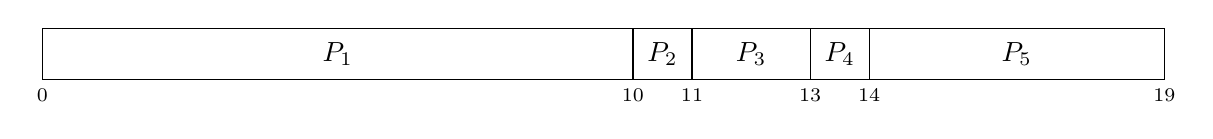
\begin{tikzpicture}[x=0.75cm,y=0.65cm]
\draw (0,0) rectangle (10,1);\node at (5.0,.5) {$P_1$};
\draw (10,0) rectangle (11,1);\node at (10.5,.5) {$P_2$};
\draw (11,0) rectangle (13,1);\node at (12.0,.5) {$P_3$};
\draw (13,0) rectangle (14,1);\node at (13.5,.5) {$P_4$};
\draw (14,0) rectangle (19,1);\node at (16.5,.5) {$P_5$};
\node[below,font=\scriptsize] at (0,0) {0};
\node[below,font=\scriptsize] at (10,0) {10};
\node[below,font=\scriptsize] at (11,0) {11};
\node[below,font=\scriptsize] at (13,0) {13};
\node[below,font=\scriptsize] at (14,0) {14};
\node[below,font=\scriptsize] at (19,0) {19};
\end{tikzpicture}\end{center}
\noindent\textbf{SJF}
\begin{center}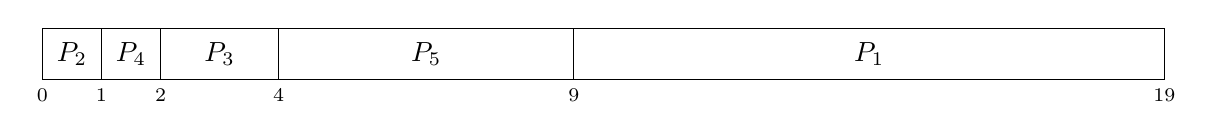
\begin{tikzpicture}[x=0.75cm,y=0.65cm]
\draw (0,0) rectangle (1,1);\node at (0.5,.5) {$P_2$};
\draw (1,0) rectangle (2,1);\node at (1.5,.5) {$P_4$};
\draw (2,0) rectangle (4,1);\node at (3.0,.5) {$P_3$};
\draw (4,0) rectangle (9,1);\node at (6.5,.5) {$P_5$};
\draw (9,0) rectangle (19,1);\node at (14.0,.5) {$P_1$};
\node[below,font=\scriptsize] at (0,0) {0};
\node[below,font=\scriptsize] at (1,0) {1};
\node[below,font=\scriptsize] at (2,0) {2};
\node[below,font=\scriptsize] at (4,0) {4};
\node[below,font=\scriptsize] at (9,0) {9};
\node[below,font=\scriptsize] at (19,0) {19};
\end{tikzpicture}\end{center}
\noindent\textbf{RR}
\begin{center}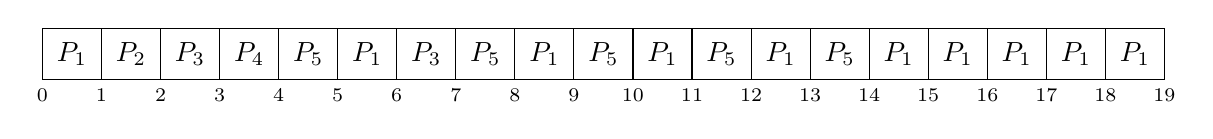
\begin{tikzpicture}[x=0.75cm,y=0.65cm]
\draw (0,0) rectangle (1,1);\node at (0.5,.5) {$P_1$};
\draw (1,0) rectangle (2,1);\node at (1.5,.5) {$P_2$};
\draw (2,0) rectangle (3,1);\node at (2.5,.5) {$P_3$};
\draw (3,0) rectangle (4,1);\node at (3.5,.5) {$P_4$};
\draw (4,0) rectangle (5,1);\node at (4.5,.5) {$P_5$};
\draw (5,0) rectangle (6,1);\node at (5.5,.5) {$P_1$};
\draw (6,0) rectangle (7,1);\node at (6.5,.5) {$P_3$};
\draw (7,0) rectangle (8,1);\node at (7.5,.5) {$P_5$};
\draw (8,0) rectangle (9,1);\node at (8.5,.5) {$P_1$};
\draw (9,0) rectangle (10,1);\node at (9.5,.5) {$P_5$};
\draw (10,0) rectangle (11,1);\node at (10.5,.5) {$P_1$};
\draw (11,0) rectangle (12,1);\node at (11.5,.5) {$P_5$};
\draw (12,0) rectangle (13,1);\node at (12.5,.5) {$P_1$};
\draw (13,0) rectangle (14,1);\node at (13.5,.5) {$P_5$};
\draw (14,0) rectangle (15,1);\node at (14.5,.5) {$P_1$};
\draw (15,0) rectangle (16,1);\node at (15.5,.5) {$P_1$};
\draw (16,0) rectangle (17,1);\node at (16.5,.5) {$P_1$};
\draw (17,0) rectangle (18,1);\node at (17.5,.5) {$P_1$};
\draw (18,0) rectangle (19,1);\node at (18.5,.5) {$P_1$};
\node[below,font=\scriptsize] at (0,0) {0};
\node[below,font=\scriptsize] at (1,0) {1};
\node[below,font=\scriptsize] at (2,0) {2};
\node[below,font=\scriptsize] at (3,0) {3};
\node[below,font=\scriptsize] at (4,0) {4};
\node[below,font=\scriptsize] at (5,0) {5};
\node[below,font=\scriptsize] at (6,0) {6};
\node[below,font=\scriptsize] at (7,0) {7};
\node[below,font=\scriptsize] at (8,0) {8};
\node[below,font=\scriptsize] at (9,0) {9};
\node[below,font=\scriptsize] at (10,0) {10};
\node[below,font=\scriptsize] at (11,0) {11};
\node[below,font=\scriptsize] at (12,0) {12};
\node[below,font=\scriptsize] at (13,0) {13};
\node[below,font=\scriptsize] at (14,0) {14};
\node[below,font=\scriptsize] at (15,0) {15};
\node[below,font=\scriptsize] at (16,0) {16};
\node[below,font=\scriptsize] at (17,0) {17};
\node[below,font=\scriptsize] at (18,0) {18};
\node[below,font=\scriptsize] at (19,0) {19};
\end{tikzpicture}\end{center}
\noindent RR ยังคงมีจุดแบ่ง quantum แม้เหลือเพียง $P_1$; จะรวมช่วงติดกันของ $P_1$ ตอนท้ายก็ได้ถ้าระบุ quantum ถูกต้อง\par\medskip
\noindent\textbf{นิยามที่ใช้}\\$T_i=C_i-A_i$; $R_i=S_i-A_i$; $W_i=T_i-B_i$ (กรณีมี CPU burst เดียว ไม่มี I/O)\\$C$: completion, $A$: arrival, $S$: first start, $B$: CPU burst\\Response time ไม่ใช่ total waiting time โดยเฉพาะเมื่อใช้ RR\par
\newpage\sectiontitle{เฉลยอัตนัยข้อ 1: ไล่ FIFO และ SJF}
\noindent\textbf{FIFO:} ทุก process มาถึงเวลาเดียวกัน ลำดับตามโจทย์จึงเป็น $P_1,P_2,P_3,P_4,P_5$. FIFO ทำงานจนจบทีละตัว ดังนั้นเวลาสิ้นสุดได้จาก burst สะสม:
\[0+10=10,\qquad 10+1=11,\qquad 11+2=13,\qquad 13+1=14,\qquad 14+5=19.\]
\begin{center}\renewcommand{\arraystretch}{1.2}\begin{tabular}{c|r|c|r|r}
Process & Burst (ms) & CPU interval & First start $S_i$ & Completion $C_i$\\\hline
$P_1$ & 10 & $[0,10)$ & 0 & 10\\
$P_2$ & 1 & $[10,11)$ & 10 & 11\\
$P_3$ & 2 & $[11,13)$ & 11 & 13\\
$P_4$ & 1 & $[13,14)$ & 13 & 14\\
$P_5$ & 5 & $[14,19)$ & 14 & 19\\
\end{tabular}\end{center}
\noindent เช่น $P_3$ เริ่มหลัง $P_1$ และ $P_2$ จบที่ $10+1=11$; ทำงาน 2 ms จึงเสร็จที่ $11+2=13$.\par\medskip
\noindent\textbf{SJF แบบไม่แทรกงาน:} เนื่องจากทุกงานพร้อมตั้งแต่ $t=0$, เลือก burst สั้นที่สุดก่อน. เรียงได้ $P_2(1),P_4(1),P_3(2),P_5(5),P_1(10)$. $P_2$ กับ $P_4$ ยาวเท่ากัน จึงใช้ลำดับมาถึงเป็น tie-break.\par
\begin{center}\renewcommand{\arraystretch}{1.2}\begin{tabular}{c|r|c|r|r}
Process & Burst (ms) & CPU interval & First start $S_i$ & Completion $C_i$\\\hline
$P_2$ & 1 & $[0,1)$ & 0 & 1\\
$P_4$ & 1 & $[1,2)$ & 1 & 2\\
$P_3$ & 2 & $[2,4)$ & 2 & 4\\
$P_5$ & 5 & $[4,9)$ & 4 & 9\\
$P_1$ & 10 & $[9,19)$ & 9 & 19\\
\end{tabular}\end{center}
\noindent ตัวอย่าง: เมื่อ $P_2$ และ $P_4$ จบที่เวลา 2, งานสั้นที่สุดที่เหลือคือ $P_3$; จึงจบที่ $2+2=4$. ทั้ง FIFO และ SJF ไม่หยุดกลาง burst ในโจทย์นี้; ตัวเลข Priority ไม่เกี่ยวกับสองนโยบายนี้.\par
\newpage\sectiontitle{เฉลยอัตนัยข้อ 1 (ต่อ): ไล่ Round Robin}
\noindent เริ่มด้วย ready queue $[P_1,P_2,P_3,P_4,P_5]$. ในแต่ละรอบหยิบหัวคิวมาใช้ CPU ไม่เกิน 1 ms. ถ้าทำเสร็จให้ออกจากระบบ; ถ้ายังเหลือ burst ให้นำไปต่อท้ายคิว. ตัวอย่างรอบแรก: $P_1$ ใช้ 1 ms จาก 10 ms เหลือ 9 ms แล้วต่อท้าย; จากนั้น $P_2$ ใช้ 1 ms จบงาน.\par\smallskip
{\small\begin{center}\renewcommand{\arraystretch}{1.12}\begin{tabular}{c|c|r|l}
เวลา (ms) & Process & Burst ที่เหลือ & ผลหลังจบ quantum\\\hline
$[0,1)$ & $P_1$ & 9 & กลับไปท้ายคิว\\
$[1,2)$ & $P_2$ & 0 & เสร็จที่ $t=2$\\
$[2,3)$ & $P_3$ & 1 & กลับไปท้ายคิว\\
$[3,4)$ & $P_4$ & 0 & เสร็จที่ $t=4$\\
$[4,5)$ & $P_5$ & 4 & กลับไปท้ายคิว\\
$[5,6)$ & $P_1$ & 8 & กลับไปท้ายคิว\\
$[6,7)$ & $P_3$ & 0 & เสร็จที่ $t=7$\\
$[7,8)$ & $P_5$ & 3 & กลับไปท้ายคิว\\
$[8,9)$ & $P_1$ & 7 & กลับไปท้ายคิว\\
$[9,10)$ & $P_5$ & 2 & กลับไปท้ายคิว\\
$[10,11)$ & $P_1$ & 6 & กลับไปท้ายคิว\\
$[11,12)$ & $P_5$ & 1 & กลับไปท้ายคิว\\
$[12,13)$ & $P_1$ & 5 & กลับไปท้ายคิว\\
$[13,14)$ & $P_5$ & 0 & เสร็จที่ $t=14$\\
$[14,15)$ & $P_1$ & 4 & เหลืองานเดียวในคิว\\
$[15,16)$ & $P_1$ & 3 & ทำต่ออีกหนึ่ง quantum\\
$[16,17)$ & $P_1$ & 2 & ทำต่ออีกหนึ่ง quantum\\
$[17,18)$ & $P_1$ & 1 & ทำต่ออีกหนึ่ง quantum\\
$[18,19)$ & $P_1$ & 0 & เสร็จที่ $t=19$\\
\end{tabular}\end{center}}
\noindent เมื่อเหลือ $P_1$ เพียงงานเดียว CPU ยังแบ่งเวลาเป็น quantum ละ 1 ms; ใน Gantt chart จะรวมช่วงท้าย $[14,19)$ เป็นกล่องเดียวก็ได้ แต่จุดแบ่งที่ 15, 16, 17 และ 18 ยังคงมีอยู่.\par

\newpage\sectiontitle{เฉลยอัตนัยข้อ 1 (ต่อ): คำนวณเวลาและค่าเฉลี่ย}
\noindent นิยามที่ใช้คือ $T_i=C_i-A_i$ และ $R_i=S_i-A_i$, โดย $S_i$ เป็นเวลาได้ CPU ครั้งแรก. ทุก process มาถึงเวลา $A_i=0$, ดังนั้น turnaround เท่ากับ completion time และ response เท่ากับ first-start time.\par\smallskip
{\small\begin{center}\renewcommand{\arraystretch}{1.12}\begin{tabular}{c|c|r|r|r|r}
Policy & Process & $S_i$ & $C_i$ & $T_i=C_i$ & $R_i=S_i$\\\hline
FIFO & $P_1$ & 0 & 10 & 10 & 0\\
 & $P_2$ & 10 & 11 & 11 & 10\\
 & $P_3$ & 11 & 13 & 13 & 11\\
 & $P_4$ & 13 & 14 & 14 & 13\\
 & $P_5$ & 14 & 19 & 19 & 14\\\hline
SJF & $P_1$ & 9 & 19 & 19 & 9\\
 & $P_2$ & 0 & 1 & 1 & 0\\
 & $P_3$ & 2 & 4 & 4 & 2\\
 & $P_4$ & 1 & 2 & 2 & 1\\
 & $P_5$ & 4 & 9 & 9 & 4\\\hline
RR & $P_1$ & 0 & 19 & 19 & 0\\
 & $P_2$ & 1 & 2 & 2 & 1\\
 & $P_3$ & 2 & 7 & 7 & 2\\
 & $P_4$ & 3 & 4 & 4 & 3\\
 & $P_5$ & 4 & 14 & 14 & 4\\
\end{tabular}\end{center}}
\noindent\textbf{ตัวอย่างแทนค่าสูตร}\\
FIFO: $P_5$ จบที่ 19 จึงได้ $T_5=19-0=19$ ms; เริ่มครั้งแรกที่ 14 จึงได้ $R_5=14-0=14$ ms.\\
RR: $P_3$ จบที่ 7 แม้ใช้ CPU รวม 2 ms จึงได้ $T_3=7-0=7$ ms; เริ่มครั้งแรกที่ 2 จึงได้ $R_3=2-0=2$ ms. เวลารอระหว่าง quantum หลังจากได้ CPU ครั้งแรกไม่ถูกนับซ้ำใน response time.\par\medskip
\newpage\sectiontitle{เฉลยอัตนัยข้อ 1 (ต่อ): ค่าเฉลี่ยและเกณฑ์ตรวจ}
\noindent\textbf{คำนวณค่าเฉลี่ย}
\begin{itemize}[leftmargin=1.4em,itemsep=.16cm]
\item FIFO: $\overline{T}=(10+11+13+14+19)/5=67/5=13.4$ ms; $\overline{R}=(0+10+11+13+14)/5=48/5=9.6$ ms.
\item SJF: $\overline{T}=(19+1+4+2+9)/5=35/5=7.0$ ms; $\overline{R}=(9+0+2+1+4)/5=16/5=3.2$ ms.
\item RR: $\overline{T}=(19+2+7+4+14)/5=46/5=9.2$ ms; $\overline{R}=(0+1+2+3+4)/5=10/5=2.0$ ms.
\end{itemize}
\noindent\textbf{สรุปข้อ (d):} SJF ให้ average turnaround ต่ำสุดที่ 7.0 ms; RR ให้ average response ต่ำสุดที่ 2.0 ms. เป็นผลเฉพาะ burst และ arrival ชุดนี้ ไม่ได้แปลว่า scheduler เดิมจะชนะทุก workload.\par\medskip
\noindent\textbf{เกณฑ์ตรวจ 8 คะแนน}
\begin{itemize}[leftmargin=1.4em,itemsep=.14cm]
\item (a) 3 คะแนน: FIFO, SJF, RR อย่างละ 1 คะแนน; ดูลำดับงานและขอบเวลาบน Gantt chart.
\item (b) 2 คะแนน: turnaround 15 ค่า; ให้ตามค่าที่คำนวณสม่ำเสมอจาก $C_i-A_i$.
\item (c) 2 คะแนน: response 15 ค่า; ใช้เวลาได้ CPU ครั้งแรก $S_i-A_i$, ไม่ใช่เวลารอรวม.
\item (d) 1 คะแนน: SJF สำหรับ minimum average turnaround (.5) และ RR สำหรับ minimum average response (.5).
\end{itemize}
\noindent หากคำนวณพลาดหนึ่งจุดแต่ใช้วิธีถูกในขั้นถัดไป ให้ follow-through credit และไม่หักความผิดเดิมซ้ำ.\par
\newpage\sectiontitle{เฉลยอัตนัยข้อ 2: MLFQ กับธนาคาร (4 คะแนน)}
\noindent\textbf{คำตอบตัวอย่างแบบเรียงความสั้น}
{\small\begin{quote}
ช่วงลูกค้าแน่น ธนาคารอาจใช้ MLFQ โดยให้ลูกค้าใหม่เริ่มคิวความสำคัญสูง และเลือกบริการจากคิวสูงสุดที่ยังมีคนรอ หากอยู่คิวเดียวกันให้ผลัดกันแบบ RR; รายการที่ยังไม่เสร็จเมื่อใช้เวลาในระดับนั้นครบจึงเลื่อนไปคิวล่างซึ่งให้ช่วงบริการยาวขึ้น และควรเลื่อนผู้ที่รอนานกลับขึ้นคิวบนเป็นระยะเพื่อไม่ให้ถูกทิ้งไว้นาน การคัดแยกรายการ เตรียมเอกสาร และเพิ่มช่องบริการตามภาระงานช่วยลดเวลาเฉลี่ยตั้งแต่เข้าคิวจนจบรายการ ทั้งนี้ควรพักธุรกรรมเฉพาะจุดปลอดภัย บันทึกความคืบหน้า และปรับนโยบายจากเวลาที่วัดได้จริง.
\end{quote}}\medskip
\noindent\textbf{แยกกฎออกมาเพื่อให้เห็นว่าใช้ MLFQ อย่างไร}
\begin{enumerate}[leftmargin=1.4em,itemsep=.18cm]
\item \textbf{เลือกคิวที่มี priority สูงสุดก่อน.} ถ้า Q0 มีลูกค้าพร้อมบริการ ให้เลือก Q0 ก่อน Q1 หรือ Q2; คิวล่างทำงานเมื่อไม่มีงานในคิวที่สูงกว่า.
\item \textbf{ใช้ RR ภายในคิวเดียวกัน.} ลูกค้าในระดับเดียวกันได้ช่วงบริการสั้น ๆ ตามลำดับ แล้ววนไปคนถัดไป จึงไม่ให้รายการเดียวครองช่องบริการตลอด.
\item \textbf{ให้รายการใหม่เริ่มคิวบนสุด.} ระบบยังไม่ทราบเวลาทำรายการจริงก่อนเริ่ม; รายการสั้นอาจจบจาก Q0 ส่วนรายการยาวจะใช้เวลาในคิวสูงต่อเนื่องมากกว่า.
\item \textbf{ลดระดับเมื่อใช้ allotment ครบ.} ถ้ารายการยังไม่จบหลังใช้เวลาสะสมครบโควตาของระดับนั้น จึงลดลงหนึ่งคิว; การ yield หรือพักก่อนหมด slice ไม่ควรล้างเวลาที่ใช้ไปแล้ว.
\item \textbf{ทำ priority boost เป็นระยะ.} เลื่อนงานที่ยังไม่เสร็จกลับขึ้นคิวสูงตามรอบ เพื่อไม่ให้งานซับซ้อนถูกงานสั้นแซงซ้ำจนแทบไม่ได้รับบริการ.
\end{enumerate}
\noindent\textbf{ตัวอย่างการเดินคิว (ตัวเลขสมมติ ไม่ใช่ค่าที่โจทย์กำหนด)}\\
พิจารณาช่องบริการเดียว มี A, B, C มาพร้อมกันและใช้เวลา 1, 5, 3 นาทีตามลำดับ; Q0 ให้ slice 2 นาทีและ Q1 ให้ slice 4 นาที.
\begin{center}\renewcommand{\arraystretch}{1.2}\begin{tabular}{c|c|l|l}
เวลา & คิว/ลูกค้า & เวลาที่เหลือ & ผล\\\hline
0--1 & Q0 / A & 0 นาที & A เสร็จที่นาที 1\\
1--3 & Q0 / B & 3 นาที & ใช้ Q0 ครบ 2 นาที จึงย้ายไป Q1\\
3--5 & Q0 / C & 1 นาที & ใช้ Q0 ครบ 2 นาที จึงย้ายไป Q1\\
5--8 & Q1 / B & 0 นาที & B ใช้ต่อ 3 นาทีและเสร็จที่นาที 8\\
8--9 & Q1 / C & 0 นาที & C ใช้ต่อ 1 นาทีและเสร็จที่นาที 9\\
\end{tabular}\end{center}
\noindent เมื่อทุกคนมาถึงเวลา 0, turnaround ของ A, B, C จึงเป็น 1, 8, 9 นาที. ตัวอย่างนี้แสดงว่าคิวสูงช่วยให้งานสั้นเสร็จเร็ว ขณะที่การลดระดับยังเปิดโอกาสให้งานยาวค่อย ๆ ทำต่อจนจบ.\par\medskip
\newpage\noindent\textbf{ข้อเสนอปรับปรุงและข้อจำกัด}
\begin{itemize}[leftmargin=1.4em,itemsep=.15cm]
\item ตรวจเอกสารและคัดประเภทบริการก่อนเข้าคิว เพื่อลดเวลาที่ช่องบริการหยุดรอข้อมูล; จัดผู้เชี่ยวชาญหรือเพิ่ม counter เฉพาะช่วงที่ข้อมูลชี้ว่าคุ้มกับกำลังคน.
\item ตั้ง slice คิวสูงสั้นพอให้งานง่ายเริ่มเร็ว แต่ไม่สั้นจนเสียเวลาเปลี่ยนงานมาก; คิวต่ำให้ช่วงยาวขึ้นเพื่อลด overhead.
\item บันทึกเวลา arrival, เริ่มบริการ, พัก, กลับมาทำต่อ และ completion แล้วคำนวณ turnaround จริงเพื่อปรับ slice, allotment และรอบ boost.
\item ธุรกรรมธนาคารหยุดสลับไม่ได้ทุกจุดเหมือน CPU: ต้องพัก ณ checkpoint ที่ปลอดภัยและเก็บ progress; หลาย counter ทำให้บริการขนานได้แต่มีต้นทุนเพิ่ม.
\end{itemize}
\noindent MLFQ ไม่รับประกัน average turnaround ต่ำที่สุดทุกชุดงานเพราะไม่ทราบเวลาบริการล่วงหน้า; ควรประเมินทั้ง turnaround, ความเป็นธรรม และความถูกต้องของธุรกรรม.\par\medskip
\noindent\textbf{เกณฑ์ตรวจ 4 คะแนน:} ความเข้าใจและการเทียบกฎ MLFQ 2 คะแนน; policy ที่นำไปใช้ได้ 1 คะแนน; ข้อเสนอปรับปรุงพร้อมเหตุผลหรือข้อจำกัด 1 คะแนน. รับตัวอย่างอื่นที่อธิบายสอดคล้อง ไม่บังคับจำนวนคิวหรือเวลาเหมือนตัวอย่างนี้.
\newpage\sectiontitle{เฉลยอัตนัยข้อ 3: Page Replacement (8 คะแนน)}
\noindent\textbf{ตาราง FIFO, LRU และ OPT (6 คะแนน)}\\
เริ่มด้วย 3 frames ว่าง; แต่ละคอลัมน์คือสถานะหลังรับ page reference นั้นแล้ว. H (hit) หมายถึง page อยู่ใน RAM อยู่ก่อน จึงไม่เปลี่ยน frame; F (fault) หมายถึง page ไม่อยู่ใน frame และต้องนำเข้ามา. เครื่องหมาย -- คือ frame ยังว่าง. ตารางย่อยจะไล่เหตุผลเฉพาะจังหวะที่ต้องเลือก victim.\par\medskip

\noindent\textbf{FIFO: 13 faults, 7 hits}
{\setlength{\tabcolsep}{5pt}\begin{center}\renewcommand{\arraystretch}{1.15}\begin{tabular}{l|cccccccccc}
Ref. no. & 1 & 2 & 3 & 4 & 5 & 6 & 7 & 8 & 9 & 10\\\hline
Page & 7 & 0 & 1 & 3 & 0 & 3 & 2 & 4 & 2 & 7\\
Frame 1 & 7 & 7 & 7 & 3 & 3 & 3 & 3 & 3 & 3 & 7\\
Frame 2 & -- & 0 & 0 & 0 & 0 & 0 & 2 & 2 & 2 & 2\\
Frame 3 & -- & -- & 1 & 1 & 1 & 1 & 1 & 4 & 4 & 4\\
H/F & F & F & F & F & H & H & F & F & H & F\\
\end{tabular}\end{center}}
{\setlength{\tabcolsep}{5pt}\begin{center}\renewcommand{\arraystretch}{1.15}\begin{tabular}{l|cccccccccc}
Ref. no. & 11 & 12 & 13 & 14 & 15 & 16 & 17 & 18 & 19 & 20\\\hline
Page & 0 & 3 & 2 & 1 & 2 & 0 & 1 & 4 & 0 & 1\\
Frame 1 & 7 & 7 & 2 & 2 & 2 & 2 & 2 & 4 & 4 & 4\\
Frame 2 & 0 & 0 & 0 & 1 & 1 & 1 & 1 & 1 & 1 & 1\\
Frame 3 & 4 & 3 & 3 & 3 & 3 & 0 & 0 & 0 & 0 & 0\\
H/F & F & F & F & F & H & F & H & F & H & H\\
\end{tabular}\end{center}}
\noindent\textbf{FIFO: ทำไมแต่ละ page จึงถูกนำออก}\quad Queue เรียงจาก page ที่เข้าก่อนสุดไปหลังสุด. References 1--3 เติม frame; เมื่อเกิด hit ลำดับ FIFO ไม่เปลี่ยน.\par\smallskip
{\small\begin{center}\renewcommand{\arraystretch}{1.12}\begin{tabular}{c|c|c|l}
Reference no. & Page เข้า & Victim & Queue หลังแทนที่ (เก่า $\rightarrow$ ใหม่)\\\hline
4 & 3 & 7 & $[0,1,3]$\\
7 & 2 & 0 & $[1,3,2]$\\
8 & 4 & 1 & $[3,2,4]$\\
10 & 7 & 3 & $[2,4,7]$\\
11 & 0 & 2 & $[4,7,0]$\\
12 & 3 & 4 & $[7,0,3]$\\
13 & 2 & 7 & $[0,3,2]$\\
14 & 1 & 0 & $[3,2,1]$\\
16 & 0 & 3 & $[2,1,0]$\\
18 & 4 & 2 & $[1,0,4]$\\
\end{tabular}\end{center}}
\noindent มี fault ตอนเติม frame 3 ครั้งแรกและ fault ที่ทำให้แทนที่อีก 10 ครั้ง รวม 13 faults; references ที่เหลือ 7 ครั้งเป็น hits.\par
\newpage\sectiontitle{เฉลยอัตนัยข้อ 3: LRU และเหตุผลเลือก victim}
\noindent LRU (Least Recently Used) แทนที่ page ที่ไม่ได้ถูกใช้นานที่สุด ณ ตอนเกิด fault. ทุก hit ต้องปรับข้อมูลว่า page นั้นเพิ่งถูกใช้; ต่างจาก FIFO ตรงที่ hit เปลี่ยนลำดับความเก่า-ใหม่ได้.\par\smallskip
\noindent\textbf{LRU: 13 faults, 7 hits}
{\setlength{\tabcolsep}{5pt}\begin{center}\renewcommand{\arraystretch}{1.15}\begin{tabular}{l|cccccccccc}
Ref. no. & 1 & 2 & 3 & 4 & 5 & 6 & 7 & 8 & 9 & 10\\\hline
Page & 7 & 0 & 1 & 3 & 0 & 3 & 2 & 4 & 2 & 7\\
Frame 1 & 7 & 7 & 7 & 3 & 3 & 3 & 3 & 3 & 3 & 7\\
Frame 2 & -- & 0 & 0 & 0 & 0 & 0 & 0 & 4 & 4 & 4\\
Frame 3 & -- & -- & 1 & 1 & 1 & 1 & 2 & 2 & 2 & 2\\
H/F & F & F & F & F & H & H & F & F & H & F\\
\end{tabular}\end{center}}
{\setlength{\tabcolsep}{5pt}\begin{center}\renewcommand{\arraystretch}{1.15}\begin{tabular}{l|cccccccccc}
Ref. no. & 11 & 12 & 13 & 14 & 15 & 16 & 17 & 18 & 19 & 20\\\hline
Page & 0 & 3 & 2 & 1 & 2 & 0 & 1 & 4 & 0 & 1\\
Frame 1 & 7 & 7 & 2 & 2 & 2 & 2 & 2 & 4 & 4 & 4\\
Frame 2 & 0 & 0 & 0 & 1 & 1 & 1 & 1 & 1 & 1 & 1\\
Frame 3 & 2 & 3 & 3 & 3 & 3 & 0 & 0 & 0 & 0 & 0\\
H/F & F & F & F & F & H & F & H & F & H & H\\
\end{tabular}\end{center}}
\noindent\textbf{ตรวจ victim ของ LRU}\quad ตัวเลขในคอลัมน์สุดท้ายคือ reference ครั้งล่าสุดที่ page นั้นถูกใช้ก่อนการแทนที่; เลือก page ที่เลขน้อยที่สุด.\par\smallskip
{\small\begin{center}\renewcommand{\arraystretch}{1.12}\begin{tabular}{c|c|c|c}
Reference no. & Page เข้า & Victim & ครั้งล่าสุดของ victim\\\hline
4 & 3 & 7 & 1\\
7 & 2 & 1 & 3\\
8 & 4 & 0 & 5\\
10 & 7 & 3 & 6\\
11 & 0 & 4 & 8\\
12 & 3 & 2 & 9\\
13 & 2 & 7 & 10\\
14 & 1 & 0 & 11\\
16 & 0 & 3 & 12\\
18 & 4 & 2 & 15\\
\end{tabular}\end{center}}
\noindent ตัวอย่างที่ reference 8: frames มี 3, 0, 2; ครั้งล่าสุดคือ 6, 5, 7 ตามลำดับ จึงแทนที่ 0 ซึ่งเก่าสุด. รวมกับ fault ตอนเติม frame ครั้งแรก 3 ครั้งจะได้ 13 faults และ 7 hits.\par
\newpage\sectiontitle{เฉลยอัตนัยข้อ 3: ตาราง OPT (ต่อ)}
\noindent OPT แทนที่ page ที่จะถูกใช้อีกครั้งช้าที่สุดในอนาคต; ถ้าไม่ถูกใช้อีกเลย ให้ถือว่าไกลที่สุด. จึงต้องมอง reference string ที่เหลือไปข้างหน้า.\par\smallskip
\noindent\textbf{OPT: 10 faults, 10 hits}
{\setlength{\tabcolsep}{5pt}\begin{center}\renewcommand{\arraystretch}{1.15}\begin{tabular}{l|cccccccccc}
Ref. no. & 1 & 2 & 3 & 4 & 5 & 6 & 7 & 8 & 9 & 10\\\hline
Page & 7 & 0 & 1 & 3 & 0 & 3 & 2 & 4 & 2 & 7\\
Frame 1 & 7 & 7 & 7 & 7 & 7 & 7 & 7 & 7 & 7 & 7\\
Frame 2 & -- & 0 & 0 & 0 & 0 & 0 & 0 & 4 & 4 & 4\\
Frame 3 & -- & -- & 1 & 3 & 3 & 3 & 2 & 2 & 2 & 2\\
H/F & F & F & F & F & H & H & F & F & H & H\\
\end{tabular}\end{center}}
{\setlength{\tabcolsep}{5pt}\begin{center}\renewcommand{\arraystretch}{1.15}\begin{tabular}{l|cccccccccc}
Ref. no. & 11 & 12 & 13 & 14 & 15 & 16 & 17 & 18 & 19 & 20\\\hline
Page & 0 & 3 & 2 & 1 & 2 & 0 & 1 & 4 & 0 & 1\\
Frame 1 & 0 & 0 & 0 & 0 & 0 & 0 & 0 & 0 & 0 & 0\\
Frame 2 & 4 & 3 & 3 & 1 & 1 & 1 & 1 & 1 & 1 & 1\\
Frame 3 & 2 & 2 & 2 & 2 & 2 & 2 & 2 & 4 & 4 & 4\\
H/F & F & F & H & F & H & H & H & F & H & H\\
\end{tabular}\end{center}}
\noindent\textbf{ไล่การตัดสินใจเมื่อ OPT เกิด fault}\\
References 1--3 เติม frame ว่าง. เลขหลัง @ คือหมายเลข reference ที่ page นั้นจะปรากฏอีกครั้ง; "ไม่มี" หมายถึงไม่ปรากฏในส่วนที่เหลือ.\par\smallskip
{\small\begin{center}\renewcommand{\arraystretch}{1.15}\begin{tabular}{c|c|c|p{5.2cm}|c}
Ref. no. & Page เข้า & Frames ก่อน fault & การใช้ครั้งถัดไปของ resident pages & Victim\\\hline
4 & 3 & $7,0,1$ & $7@10,\ 0@5,\ 1@14$ & 1\\
7 & 2 & $7,0,3$ & $7@10,\ 0@11,\ 3@12$ & 3\\
8 & 4 & $7,0,2$ & $7@10,\ 0@11,\ 2@9$ & 0\\
11 & 0 & $7,4,2$ & $7$ ไม่มี, $4@18,\ 2@13$ & 7\\
12 & 3 & $0,4,2$ & $0@16,\ 4@18,\ 2@13$ & 4\\
14 & 1 & $0,3,2$ & $0@16,\ 3$ ไม่มี, $2@15$ & 3\\
18 & 4 & $0,1,2$ & $0@19,\ 1@20,\ 2$ ไม่มี & 2\\
\end{tabular}\end{center}}
\noindent ตัวอย่างที่ reference 4: จาก frames $7,0,1$ นั้น 7 จะกลับมาใช้ที่ 10, 0 ที่ 5 และ 1 ที่ 14; จึงนำ 1 ออกเพราะต้องรอนานที่สุด. OPT ได้ 3 faults ตอนเติม frame และอีก 7 faults ตามตาราง รวม 10 faults; ที่เหลือเป็น 10 hits. หากมี tie ระหว่าง page ที่ไม่ถูกใช้อีก เลือก victim ตัวใดก็ได้ที่ให้ผล optimal.\par
\newpage\sectiontitle{เฉลยอัตนัยข้อ 3 (ต่อ): EAT และเกณฑ์ตรวจ}
\noindent\textbf{ขั้นที่ 1: ทำหน่วยให้ตรงกัน}\\
Memory access time $m=10$ ns $=0.00001$ ms. Disk access time $D=10$ ms $=10{,}000{,}000$ ns. จะใช้หน่วย ns ทั้งหมดหรือแปลงเป็น ms ทั้งหมดก็ได้ แต่ห้ามบวก ns กับ ms โดยตรง.\par\medskip
\noindent\textbf{ขั้นที่ 2: หาโอกาส hit และ fault}\\
มี references ทั้งหมด 20 ครั้ง. ให้ $p=\text{faults}/20$ เป็นโอกาสเกิด page fault และ $h=\text{hits}/20=1-p$ เป็นโอกาส hit. ใช้โมเดล Lecture 6:
\[\mathrm{EAT}=hm+pD=(1-p)m+pD.\]
\noindent ในที่นี้ $D$ แทน disk access time ตามที่โจทย์ให้; ไม่เพิ่มต้นทุนอื่นที่โจทย์ไม่ได้ระบุ.\par\medskip
\noindent\textbf{ขั้นที่ 3: แทนค่าและคำนวณ}
\begin{itemize}[leftmargin=1.4em,itemsep=.2cm]
\item \textbf{FIFO:} $p=13/20=0.65$ และ $h=7/20=0.35$.\\
$\mathrm{EAT}=0.35(10\,\mathrm{ns})+0.65(10{,}000{,}000\,\mathrm{ns})$\\
$=3.5+6{,}500{,}000=6{,}500{,}003.5$ ns $=6.5000035$ ms $\approx 6.5$ ms.
\item \textbf{LRU:} fault/hit counts เท่ากับ FIFO สำหรับ string นี้, จึง $p=0.65$, $h=0.35$ และ EAT $=6{,}500{,}003.5$ ns $=6.5000035$ ms $\approx 6.5$ ms.
\item \textbf{OPT:} $p=10/20=0.5$ และ $h=10/20=0.5$.\\
$\mathrm{EAT}=0.5(10\,\mathrm{ns})+0.5(10{,}000{,}000\,\mathrm{ns})$\\
$=5+5{,}000{,}000=5{,}000{,}005$ ns $=5.000005$ ms $\approx 5.0$ ms.
\end{itemize}
\noindent\textbf{สรุปผล}
\begin{center}\renewcommand{\arraystretch}{1.2}\begin{tabular}{l|r|r|r|l}
Policy & Faults & Hits & $p$ & EAT\\\hline
FIFO & 13 & 7 & 0.65 & $6.5000035$ ms\\
LRU & 13 & 7 & 0.65 & $6.5000035$ ms\\
OPT & 10 & 10 & 0.50 & $5.0000050$ ms\\
\end{tabular}\end{center}
\noindent OPT ให้ EAT ต่ำสุดในชุดนี้เพราะมี page faults น้อยที่สุด; FIFO กับ LRU ได้จำนวน fault เท่ากันโดยบังเอิญจาก reference string นี้ ไม่ได้แปลว่าจะเท่ากันทุกชุด. ถ้ารายงานโดยปัดเลข ได้ประมาณ 6.5 ms สำหรับ FIFO/LRU และ 5.0 ms สำหรับ OPT.\par\medskip
\noindent\textbf{Rubric รวม 8 คะแนน}
\begin{itemize}[leftmargin=1.4em,itemsep=.18cm]
\item ตาราง frames รวม 6 คะแนน: แต่ละ policy 2 คะแนน ให้ตาม frame contents 20 คอลัมน์ คอลัมน์ละ .1; ไม่หักเพราะไม่มีแถว hit/fault หรือการรายงาน counts แยกต่างหาก
\item EAT รวม 2 คะแนน: สูตร .5; แปลงหน่วย .5; EAT แต่ละ policy ค่าละ $1/3$ ไม่บังคับเขียนข้อสรุปเพิ่มเติมที่โจทย์ไม่ได้ถาม
\end{itemize}
\noindent ให้ follow-through credit สำหรับ EAT ที่ใช้จำนวน fault จากตารางของผู้สอบอย่างถูกวิธี แม้ตารางก่อนหน้าผิด โดยหักข้อผิดเดิมในตาราง/จำนวน faults; ต้องไม่ให้คะแนนเต็มหากแทนค่าคนละหน่วยในสมการเดียวกัน
\newpage\sectiontitle{แผนผังเนื้อหาและแหล่งอ้างอิงสำหรับตรวจทบทวน}
\noindent\textbf{ความครอบคลุมของปรนัย}

\begin{center}\renewcommand{\arraystretch}{1.15}\begin{tabular}{lcl}
Lecture & จำนวนปรนัย & หัวข้อ\\\hline
1 & 3 & Privilege, trap, isolation\\
2 & 14 & Process, state, context switch, wait\\
3 & 8 & FIFO/SJF/STCF/RR, MLFQ, metrics\\
4 & 3 & C storage class, partition fragmentation\\
5 & 7 & Segmentation, paging, address translation\\
6 & 6 & Virtual memory, demand paging, replacement\\
\end{tabular}\end{center}
\noindent\textbf{แหล่งเนื้อหา (path เทียบกับ root ของ repository)}
\begin{itemize}[leftmargin=1.4em,itemsep=.18cm]
\item lectures/CPE333\_OS\_Midterm\_StudyNotes.pdf และ Lecture1--Lecture6: ใช้กำหนดขอบเขต ไม่รวม threads/locks/deadlock ที่อยู่นอกชุด Lecture 1--6
\item ปรนัย 1 ข้ออิงข้อสอบ CPE326 ปี 2561 (E03, ข้อ 7) และ 40 ข้ออิงชุดคำถามปี 2022 (E09); ตรวจตัวเลือกที่ไหลต่อข้ามหน้าจากไฟล์เต็ม 16 หน้า และใช้ Lecture 1--6 ตัดสินเฉลยเมื่อ annotation ขัดกับเนื้อหา
\item quiz-and-exam/midterm/Backroom.pdf และข้อสอบปี 2558/2561: เทียบหัวข้อและแนวคำถาม ไม่คัดลอกหน้าที่มีคำตอบเขียนกำกับ; เมื่อเครื่องหมายเฉลยขัดกับ Lecture ให้ยึดแนวคิดใน Lecture (เช่น E09 Q6 และ Q24)
\item quiz-and-exam/midterm/ยำรวมมิตรข้อเขียน.pdf หน้า 4--6 และ 10: Scheduling, bank analogy และ MLFQ rules; ตัวเลข burst ใช้ 10,1,2,1,5 รวม 19 ms ตามโจทย์ชุดนี้ ไม่ใช่ Quiz อีกชุดที่ $P_4=2$
\item E09: \texttt{os midterm exam.pdf} หน้า 1--16 เป็น bank ปรนัยฉบับเต็ม; ตรวจภาพครบทุกหน้าและตามตัวเลือกที่ไหลข้ามหน้าใน Q4, Q7, Q10, Q17, Q20, Q27, Q30, Q40, Q43 และ Q50. E05 เป็นไฟล์สรุป quiz ปี 2022 ซึ่งมีเฉลยถึง Q40 แต่ไม่มีชุดตัวเลือกครบ
\item E09 Q15 ใช้โดยระบุให้ชัดว่าเรียงตามลำดับการทำงานจนเสร็จ จึงตอบ FIFO; ตัวเลือก ``Both FIFO and RR'' คงตามต้นฉบับ แต่ไม่ได้ใช้เป็นเฉลยของ stem ที่ปรับให้แคบลง. Q45 ซ้ำกับ Q44 และตัดข้อที่อยู่นอกขอบเขตหรือยังมีคำตอบกำกวมออก
\item quiz-and-exam/midterm/Quiz\_BeforeMidterm.pdf: เทียบรูปแบบโจทย์ Scheduling และ fit policy
\end{itemize}
\noindent\textbf{แม่แบบการพิมพ์}\\
Palapluem/cpe222-past-exam-main, commit e87b379d09fdeb54f964d968c9599efdea68ba5d; main wrapper, cover และ chapter templates\\
คงการประกอบ PDF, ฟอนต์ THSarabunNew, margin, student header และกล่องหน้าปก; บรรทัดดอกจันบนปกใช้ข้อความตามแม่แบบที่ผู้ใช้ขอ ไม่ใช่การตรวจยืนยันการรับรองจริง
\par\medskip
\noindent วันและเวลาตามข้อมูลที่ผู้ใช้ให้: 26 ตุลาคม 2569, 09.00--12.00 น. รายละเอียดคะแนนย่อยและเฉลยเป็นเกณฑ์ฝึกซ้อมแยกเล่ม แหล่งข้อสอบเก่าที่ใช้ระบุไว้ข้างต้น
